%%
% BIThesis 本科毕业设计论文模板 —— 使用 XeLaTeX 编译 The BIThesis Template for Undergraduate Thesis
% This file has no copyright assigned and is placed in the Public Domain.
% Compile with: xelatex -> biber -> xelatex -> xelatex
%%

% 请勿删除下面两行注释,以免影响编译。
% !TeX program = xelatex
% !BIB program = biber


% 开启盲审格式 blindPeerReview=true (如:[type=bachelor,blindPeerReview=true])

\documentclass[type=bachelor]{bithesis}

% 此处仅列出常用的配置。全部配置用法请见「bithesis.pdf」手册。
\BITSetup{
  cover = {
    % 封面需要「北京理工大学」字样图片,如无必要请勿修改该项。
    headerImage = images/header.png,
    % 封面标题需要“华文细黑”,如无必要请勿修改该项。
    xiheiFont = STXIHEI.TTF,
    % 可用以下参数自定义封面日期。
    % date = 1955年11月,
  },
  info = {
    % 想要删除某项封面信息,直接删除该项即可。
    % 想要让某项封面信息留空(但是保留下划线),请传入空白符组成的字符串,如"{~}"。
    % 如需要换行,则用 “\\” 符号分割。
    title = 基于强化学习的对抗性恶意程序生成方法研究,
    titleEn = {Reinforcement Learning-Based Adversarial Malicious Sample Generation Method},
    school = 计算机学院,
    major = 计算机科学与技术,
    class = 07112105,
    author = 李函书,
    studentId = 1120213139,
    supervisor = 田东海,
    keywords = {强化学习;静态分析规避;PE恶意可执行文件},
    keywordsEn = { Reinforcement learning; Static analysis evasion; PE malicious executable},
    % 如果你的毕设为校外毕设,请将下面这一行语句解除注释(删除第一个百分号字符)并填写你的校外毕设导师名字
    % externalSupervisor = 左偏树,
  },
  style = {
    % 开启 Windows 平台下的中易宋体伪粗体。
    % windowsSimSunFakeBold = true,
    %
    % 开启该选项后,将用 Times New Roman 的开源字体 TeX Gyre Termes 作为正文字体。
    % 这个选项适用于以下情况:
    % 1. 不想在系统中安装 Times New Roman。
    % 2. 在 Linux/macOS 下遇到 `\textsc` 无法正常显示的问题。
    % betterTimesNewRoman = true,
  },
  misc = {
    % 微调表格行间距
    tabularRowSeparation = 1.25,
  },
}

% 这份模板提供了代码块示例,采用 listings 宏包及其预定义样式。
% 使用代码块时,也可选用自己的喜欢的其他宏包,如 minted:https://bithesis.bitnp.net/faq/minted.html
% 如果不需要,直接删除即可。
\usepackage{listings}


% 大部分关于参考文献样式的修改,都可以通过此处的选项进行配置。
% 详情请搜索「biblatex-gb7714-2015 文档」进行阅读。
\usepackage[
  backend=biber,
  style=gb7714-2015,
  gbalign=gb7714-2015,
  gbnamefmt=lowercase,
  gbpub=false,
  doi=false,
  url=false,
  eprint=false,
  isbn=false,
]{biblatex}

% 参考文献引用文件位于 misc/ref.bib
\addbibresource{misc/ref.bib}

% 若要按计算机学院要求,添加“北京理工大学”水印,请参考
% https://bithesis.bitnp.net/faq/watermark.html

% 文档开始
\begin{document}

% 标题页面:如无特殊需要,本部分无需改动
\MakeCover

% 原创性声明:盲审结束前无需改动
% 后续添加签名时,可考虑先用 Word 制作再覆盖 misc/1_originality.pdf。
% 不过如无特殊需要,本部分的代码仍无需改动。
\begin{blindPeerReview}
  
\includepdf{misc/1_originality.pdf}\newpage
\end{blindPeerReview}
% %%
% BIThesis 本科毕业设计论文模板 —— 使用 XeLaTeX 编译 The BIThesis Template for Undergraduate Thesis
% This file has no copyright assigned and is placed in the Public Domain.
%%

% 如无特殊需要,本页面无需更改

\MakeOriginality


% 前置内容定义
\frontmatter
% 摘要:在相应 TeX 文件撰写
%%
% BIThesis 本科毕业设计论文模板 —— 使用 XeLaTeX 编译 The BIThesis Template for Undergraduate Thesis
% This file has no copyright assigned and is placed in the Public Domain.
%%

% 中英文摘要章节
\begin{abstract}
% 中文摘要正文从这里开始

\textcolor{black}{近年来,随着勒索病毒和恶意PE可执行文件木马程序的流行,目前存在的一些反病毒软件的查杀引擎,例如360杀毒使用的基于机器学习的QVM引擎,对于恶意PE可执行文件的检测仍然有较多的漏报和误报问题,反病毒软件厂商为了解决漏报和误报问题,需要用户主动向反病毒软件的维护人员提交漏报样本和误报样本,但这无疑存在效率较低的问题。同时,部分反病毒软件过度依赖动态检测来对抗恶意软件,静态检测能力不足,难以做到在恶意软件刚出现但是没有被运行时隔离恶意软件。}

\textcolor{black}{为了提供静态对抗性恶意样本供反病毒软件训练,本文提出并实现了一种基于强化学习的Sarsa算法的静态对抗型样本生成框架,输入为PE可执行程序恶意样本集合,输出为能够规避部分反病毒软件静态检测的对抗性样本,其由三个模块组成,分别是样本筛选模块、恶意程序扫描模块、强化学习对抗性样本生成模块。样本筛选模块实现了对于收集到的样本的处理,删除不符合条件的样本,最终生成原始样本。恶意程序扫描模块实现了获取样本集处理前后的检出率,以及判定经过强化学习对抗性样本生成模块处理后的样本能否逃逸静态检测。强化学习对抗性样本生成模块由筛选后的样本和指定的行为集和参数生成能够逃逸静态检测的对抗性样本。在实验中,某个样本集经处理前后,Clam AV对其查杀率从31.3\%下降到了20.7\%,360杀毒对其的查杀率从99.1\%下降到了4.2\%。总而言之,使用本文中提出的方法生成的静态对抗样本集对反病毒软件进行训练,可以提高基于深度学习和机器学习的反病毒软件的对于恶意软件的检测能力,对恶意PE可执行文件检测的攻防对抗领域有一定的贡献。同时本模型不同于已存在的psp-mal模型,创新点在于使用了仍在更新的ClamAV反病毒软件,360杀毒等作为静态规避检测标准,而非已经过时的EMBER反病毒模型,保证了对于更流行的反病毒软件的规避。并且引入了基于文件大小变化的奖励修正,鼓励生成更小的对抗性样本。最后,操作集相比psp-mal的操作集新增了UPX加壳,图标资源增加,签名伪造等更多操作,增加了可迁移性。}

%\textcolor{blue}{摘要正文选用模板中的样式所定义的“正文”,每段落首行缩进 2 个字符;或者手动设置成每段落首行缩进 2 个汉字,字体:宋体,字号:小四,行距:固定值 22 磅,间距:段前、段后均为 0 行。阅后删除此段。}

%\textcolor{blue}{摘要是一篇具有独立性和完整性的短文,应概括而扼要地反映出本论文的主要内容。包括研究目的、研究方法、研究结果和结论等,特别要突出研究结果和结论。中文摘要力求语言精炼准确,本科生毕业设计(论文)摘要建议 300-500 字。摘要中不可出现参考文献、图、表、化学结构式、非公知公用的符号和术语。英文摘要与中文摘要的内容应一致。阅后删除此段。}

\end{abstract}

% 如需手动控制换行连字符位置,可写 aa\-bb,详见
% https://bithesis.bitnp.net/faq/hyphen.html

% 英文摘要章节
\begin{abstractEn}
% 英文摘要正文从这里开始
%In order to study……

%\textcolor{blue}{Abstract 正文设置成每段落首行缩进 2 字符,字体:Times New Roman,字号:小四,行距:固定值 22 磅,间距:段前、段后均为 0 行。阅后删除此段。}
\textcolor{black}{In recent years, with the prevalence of ransomware and malicious Portable Executable programs, most antivirus engines—such as the QVM engine, which is based on machine learning and is used by 360 Anti-Virus—still exists tremendous false negatives and false positives in malicious PE executables detection. To solve these issues, antivirus software developers require users to actively submit samples which are malicious but not detected by antivirus software or are benign but software regard them as malware to their maintenance teams, which is inefficient. Additionally, some antivirus software excessively relies on dynamic detection to identify malware, which results in deficient static detection capabilities and has difficulty in quarantining newly emerged malware before it is executed by user.}

\textcolor{black}{To provide static adversarial samples for antivirus systems training whose purpose is detecting malware more accurately, this project raises and creates a static adversarial sample generation framework which is based on reinforcement learning Sarsa algorithm. The framework which consists of three modules: sample swifting module, malware scanning module, and reinforcement learning adversarial sample generation module, needs malicious PE executable samples as input, after processing, it outputs adversarial samples which can evade static detection of some antivirus software. The sample swifting module implements the processing of samples by removing samples which do not fit this experiment. The malware scanning module calculates detection rates of sample sets before and after processing, besides,it  determinines whether samples which are processed by the reinforcement learning adversarial sample generation module can evade static detection. The reinforcement learning adversarial sample generation module generates adversarial samples which can evade static detection by using origin samples and specified behavior sets and parameters.The experiment shows the result that after processing a sample set, the detection rate by Clam AV dropped from 31.3\% to 20.7\%, while the detection rate of 360 Anti-Virus’s declined from 99.1\% to 4.2\%.Generally, training antivirus software with the static adversarial samples which are generated by the reinforcement model can enhance the malware detection capabilities of antivirus software and engines which are based on deep learning and machine learning. This experiment contributes to the defensive domain of malicious PE executable detection. Moreover, this model innovations make this model differ from the existing PSP-Mal framework.Firstly, it adopts actively updated antivirus engines such as ClamAV and 360 Anti-Virus as static evasion detection standard,which replaces the outdated EMBER antivirus model,  ensures evasion effectiveness against prevalent anti-virus software. Secondly, a reward adjustment method which is modified by the change of file size is adopted to encourage the generation of smaller adversarial samples. Secondly, the operation set has been expanded,which is different from PSP-Mal's original configuration ,contains UPX packing, icon resource modification, and signature fabrication techniques, enhances the transferability.}
\end{abstractEn}


\MakeTOC

% 正文开始
\mainmatter

% 在这里引用各章 TeX 文件,按需添加

%%
% BIThesis 本科毕业设计论文模板 —— 使用 XeLaTeX 编译 The BIThesis Template for Undergraduate Thesis
% This file has no copyright assigned and is placed in the Public Domain.
%%

% 第一章节
\chapter{引言}

\section{研究背景和意义}

\textcolor{black}{恶意软件是经过精心设计,被用来攻击计算机系统或计算机网络并且造成损害的软件,危害不仅限于感染型病毒和蠕虫的自身复制耗尽系统资源,破坏操作系统、后门软件开放系统端口供黑客连接从而形成僵尸网络对服务器发起分布式拒绝服务攻击、木马伪装成正常程序,实则窃取用户的敏感数据和破坏系统,为黑客提供后门、勒索病毒加密文件要求用户支付赎金等。根据统计数据,仅2022年在全球大约发生了55亿次恶意软件攻击事件\parencite{ref1}。}

\textcolor{black}{在早期,恶意软件的代码较为简单,容易被反病毒软件检测到特征值从而处理清除。但是多年以来,恶意软件的复杂性不断发展,传统的基于黑名单哈希值的恶意软件检测技术难以应对当今恶意软件复杂的混淆策略,尽管这种方法速度很快,但是难以识别新一代的恶意软件以及一些0day恶意软件\parencite{ref2}。}

\textcolor{black}{目前,为了应对恶意软件带来的威胁,许多开源以及商业杀毒软件厂商不断升级病毒库,更替杀毒软件版本。目前针对恶意软件的识别主要分为静态分析、动态分析以及混合分析(同时结合了静态分析和动态分析)这三种。而本实验研究的强化学习模型,是生成针对反病毒软件的静态特征分析的PE可执行程序对抗性样本,目的是用于反病毒软件厂商的机器学习和深度学习反病毒引擎模型训练和逆向分析工作者们学习研究,本实验未研究动态特征分析对抗性样本生成。静态特征分析包括文件Hash(如MD5 SHA256)匹配,这在很多病毒样本分析网站,例如VirusTotal,VirusSCAN等被使用,如果上传的文件和病毒库里面存在的样本的Hash值匹配,则反病毒软件判断该文件是病毒。此外,静态分析还包括资源节分析,时间戳检查,数字签名检查,函数导入表检查,特征字符串匹配,DEBUG信息检查等。}

\textcolor{black}{在过去的十几年中,学术界出现了大量利用机器学习和强化学习的恶意软件查杀模型判断恶意软件的研究成果,甚至可以运用启发式杀毒规则,检测分析软件的代码行为,来判断从未出现过的新型恶意软件\parencite{ref3},\parencite{ref4},\parencite{ref5},\parencite{ref6},\parencite{ref7},\parencite{ref8}。}

\textcolor{black}{但不幸的是,某些基于静态特征分析的反病毒软件在某些情况下有着很高的误报率,可能因为机器学习模型自身的问题,误判一些正常的软件的行为,认为这些正常软件是恶意软件,例如QVM反病毒引擎误报Microsoft Visual Studio Complier、Clang等C/C++语言编译器,以及LLVM语法分析器等软件。此外,基于机器学习的反病毒软件也存在严重的漏洞,攻击者只需要对恶意软件进行修改,甚至有时只需要增加一个资源文件改变恶意软件的Hash值,就能绕过反病毒软件的检测,恶意软件的编写者的规避技术对于反病毒软件的识别带来了极大的挑战,这促使攻防对抗的双方不断采取更先进的措施。}

\section{国内外对于对抗性样本生成研究现状}

\textcolor{black}{在过往的PE对抗性样本生成实验中,许多已有的对抗性模型生成,有些采用值函数的强化学习算法,例如使用深度学习神经网络的DQN\parencite{ref9}。}

\textcolor{black}{有些使用遗传编程算法,基于适应度进行选择,交叉,编译\parencite{ref10}。}

\textcolor{black}{有些采用蒙特卡洛搜索树方法,将对抗样本转化为路径搜索问题\parencite{ref11}。}

\textcolor{black}{这些现有的方法已经展现了一定有效性,但时序差分算法,例如Sarsa或Q-learning的研究却很稀少,因此本实验的主要研究目标是使用时序差分算法Sarsa构建强化学习对抗性样本生成模型,来生成能够规避部分静态检测的PE可执行程序对抗样本,使部分样本逃逸反病毒软件的查杀。}

\textcolor{black}{基于强化学习的方法是通过构建动作(Action),状态(State),奖励(Reward),来使智能体与环境交互,通过多次操作获取经验,挑选一个相对更好的策略来修改已有的PE恶意程序来达到逃逸反病毒软件检测。}

\textcolor{black}{在2017年,基于强化学习生成静态对抗性样本绕过黑盒的反病毒软件的GYM-Malware框架被提出。Anderson等人定义了10种不会影响恶意软件和功能的扰动操作,例如利用签名漏洞来更改恶意软件的签名,修改恶意软件的调试(Debug)信息,修改可选首部检验码(checksum),修改现有的节的名称。这些操作与DQN强化学习算法结合和病毒检测软件交互以指导选择的扰动操作\parencite{ref9},\parencite{ref13}。}

\textcolor{black}{但遗憾的是,一部分使用强化学习模型生成的对抗性样本无法在虚拟机中正常执行,有一部分恶意软件经过某些操作后被破坏了。尽管某些操作修改的部分似乎与恶意软件的代码部分无关,但还是影响到了恶意程序的功能\parencite{ref8}。}

\textcolor{black}{但GYM-Malware模型仍然对后续的研究有着很大的作用,许多后续的研究基于其工作来进行。其中封装的一部分动作(Action),被拆成了函数用于其他的研究中,例如Mab-malware。}

\textcolor{black}{有一些研究\parencite{ref14},关注了GYM-Malware中的一些造成恶意软件功能损坏无法正常执行的操作。Mab-Malware认为是Python的LIEF库导致的,并且对其进行修复,将使用LIEF库的一些对PE可执行程序的操作改为使用Python的Pefile库,以减少损坏的恶意程序数量。也有一些研究\parencite{ref15},直接删除了可能导致恶意程序遭到破坏的操作,引入随机化操作来缩小动作空间,限制强化学习智能体可执行的动作次数,鼓励强化学习智能体寻找更优秀的Action集合。}

\textcolor{black}{而由Labaca-Castro等人开展的研究\parencite{ref16},则考虑修正奖励函数,对奖励函数添加惩罚因子,为了进一步优化强化学习智能体的操作。对奖励函数的修正鼓励智能体尽可能用更少的步骤对恶意PE程序进行修改以逃逸反病毒软件的检测。}

\textcolor{black}{类似的,Gibert et al.等人使用空操作\parencite{ref17},即插入大量NOP指令来修改恶意软件,表明使用插入无意义空操作的方法对于绕过MalConv等反病毒软件一样是有效的。}

\textcolor{black}{同时,目前也存在基于梯度的对抗性样本生成,例如FGSM、 Carlini和Wagner创建的C\&W、以及deepfool模型\parencite{ref18},\parencite{ref19},\parencite{ref20}。}

\textcolor{black}{且存在一些研究能够在已知梯度信息的情况下,通过基于梯度的方法对恶意软件的字节或者外观表现形式进行修改来规避静态特征检测\parencite{ref21},\parencite{ref22},\parencite{ref23},\parencite{ref24},\parencite{ref25},\parencite{ref26}。}

\section{创新点及主要工作贡献}
\subsection{创新点}

\textcolor{black}{本实验采用的强化学习算法是基于时序查分算法的Sarsa算法。关注PE恶意程序的原因是Windows操作系统在个人电脑(PC),服务器等操作系统中占有72\%左右的份额,因此超过70\%的恶意软件将Windows操作系统作为攻击目标\parencite{ref27},\parencite{ref28}。相比已有的工作,本实验额外考虑了UPX加壳操作和sigthief造成的假数字签名,resourceHacker调用导致的图标类资源添加等行为,对静态检测的对抗性样本生成可能带来的影响。同时,使用了仍在更新的ClamAV反病毒软件,360杀毒等作为静态规避检测标准,而非已经过时的EMBER反病毒模型,保证了对于更流行的反病毒软件的规避。并且引入了基于文件大小变化的奖励修正,鼓励生成更小的对抗性样本。最后,生成的对抗性样本相比psp-mal,增加了可迁移性。}

\subsection{主要工作贡献}

\textcolor{black}{本文的主要贡献如下:}

\textcolor{black}{(1)研究了时序差分强化学习算法Sarsa对于对抗性样本的生成。}

\textcolor{black}{(2)能够生成高概率逃逸360杀毒云查杀的对抗性样本并且保证恶意程序的功能,生成的恶意程序样本即使开启了允许上传可疑文件,仍然需要经过多次扫描后上传分析才得以查杀。}

\textcolor{black}{(3)预测了未来可能出现的高危害性感染型病毒变种和结合了静态分析的挂马网站,以及部分木马下载器变种,并且建议反病毒软件厂商们加以防范,尽管动态分析技术仍然可以针对感染型病毒变种,但该类型病毒仍具有一定威胁性。这种感染型病毒变种会在感染新文件时对于新产生的病毒自带进行自动地静态检测规避处理,同时被感染的文件相较于传统的感染型病毒难以恢复。}

\textcolor{black}{(4)Action更加倾向于模块化,减少了模块之间的耦合程度,便于后续的研究人员从项目中直接提取函数,而无需修改大量内容,对于某些扰动函数只需要传入原恶意程序文件的绝对路径,和用户期望生成的文件的绝对路径,就能实现对抗型扰动操作。相比原有框架PSP-Mal\parencite{ref12},本实验项目中的扰动函数与行为(Action)相互分离,并且额外加入日志系统,扰动函数自身不需要传递过多的参数。而原框架PSP-Mal对于恶意软件的操作相对混乱,难以单独从一个行为(Action中)抽象出修改函数,对恶意软件的扰动行为和智能体之间耦合度过高,导致修改较为困难。}

\section{论文结构}
\textcolor{black}{本文第一章为引言部分,说明了本课题的研究背景和意义,介绍恶意软件检测技术的研究现状,并且简要说明了工作的内容和创新点。第二章研究了本课题相关工作的PE文件结构及强化学习算法的相关理论性知识。第三章介绍实验的各个模块的功能的设计和实现。第四章是本文的实验部分以及运行环境配置的具体过程。第五章分析结果以及提出实验中预测的未来潜在威胁恶意软件以及对于相关方向人员的一些建议。在结论中总结了本文的成果和工作的创新点,提出了工作中存在的问题以及未来的可选修改方向。}
%%
% BIThesis 本科毕业设计论文模板 —— 使用 XeLaTeX 编译 The BIThesis Template for Undergraduate Thesis
% This file has no copyright assigned and is placed in the Public Domain.
%%

% 第一章节
\chapter{预备知识}

\section{实验预备知识}

\subsection{PE文件}

\textcolor{black}{PE文件是Windows操作系统下的可执行文件形式,包括EXE(可执行文件),DLL(动态链接库),SYS(系统文件)等类型。}

\textcolor{black}{PE文件中包含PE文件头(IMAGE\_NT\_HEADERS),其中的COFF文件头(IMAGE\_FILE\_HEADER)和可选首部(IMAGE\_OPTIONAL\_HEADER)中的有些部分是我们需要修改的目标。}]

\textcolor{black}{COFF文件头(IMAGE\_FILE\_HEADER)包含如下关键字段:}

\textcolor{black}{(1)Machine:目标CPU架构,指明了能运行这个程序的机器码,可以指明支持程序运行的机器架构是x86、x64、PowerPC、ARM等。}

\textcolor{black}{(2)NumberOfSections:指明所有节区的数量。}

\textcolor{black}{(3)TimeDateStamp:时间戳,指明了这个文件被编译生成的时间。}

\textcolor{black}{(4)SizeOfOptionalHeader:可选首部的大小。}

\textcolor{black}{(5)Characteristics:文件的类型,是动态链接库,还是可执行文件等类型。}

\textcolor{black}{可选首部(IMAGE\_OPTIONAL\_HEADER)包含如下字段,可选首部指明了当PE程序被载入内存后的一些情况:}

\textcolor{black}{(1)Magic:魔法位,包含PE信息,一定要和COFF文件头中的Machine对应,否则就会报错导致程序无法启动。}

\textcolor{black}{(2)AddressOfEntryPoint:程序入口点,即相对虚拟地址。}

\textcolor{black}{(3)ImageBase:加载机制。}

\textcolor{black}{(4)SectionAlignment:内存中节区的对齐粒度,不建议修改,否则程序可能无法启动。}

\textcolor{black}{(5)FileAlignment:文件中节区的对齐粒度,不建议修改,否则程序将无法启动。}

\textcolor{black}{(6)SizeOfImage:加载到内存后的总大小。}

\textcolor{black}{(7)SubSystem:子系统类型。}

\textcolor{black}{(8)DataDirectory:数据目录表,记录某些数据的位置及其大小。}

\textcolor{black}{PE文件中的节表(Section table)描述了每个节的属性,由多个IMAGE\_SECTION\_HEADER组成,每个条目对应一个节区,包括下列关键属性:}

\textcolor{black}{(1)Name:节区的名字。}

\textcolor{black}{(2)VirtualAddress:虚拟地址中的起始相对位置。}

\textcolor{black}{(3)SizeOfRawData:节区中数据的大小。}

\textcolor{black}{(4)PointerToRawData:节区偏移量。}

\textcolor{black}{(5)Characteristics:节区属性。}

\textcolor{black}{节区数据正常情况下应包含如下内容:}

\textcolor{black}{(1).text:代码节,存放该PE程序执行的指令。}

\textcolor{black}{(2).data:已经完成初始化的某些数据。}

\textcolor{black}{(3).rdata:只读(Read Only)的数据。}

\textcolor{black}{(4).rsrc:资源节,存放PE文件的图标等信息。}

\textcolor{black}{(5).reloc:重定位信息,可以用于动态链接库的装载过程。}

\textcolor{black}{(6).idata:import data,即导入函数信息。}

\textcolor{black}{数据目录表中包含的内容如下:}

\textcolor{black}{(1)Import Table:导入表,用于存放该PE文件依赖的动态链接库和调用的某些函数。}

\textcolor{black}{(2)Export Table:导出表,可以用于存放这个PE文件封装好的函数,多半运用于动态链接库封装函数供其余PE程序调用使用。}

\textcolor{black}{(3)Relocation Table:重定位表,修复地址偏移相关问题。}

\textcolor{black}{(4)TLS:线程存储表,与多线程程序有关,存储线程初始化数据。}

\textcolor{black}{(5)Debug Directory:存放该PE程序的调试信息。}

\subsection{强化学习}

\textcolor{black}{基本概念相关:}

\textcolor{black}{(1)智能体:在强化学习中决策,行动,学习。智能体是一个感知者,能感知并且理解当前的状态,智能体是一个决策者,能够知道在一个状态下应该采取什么行动,智能体是一个执行者,通过改变状态从而获取奖励。}

\textcolor{black}{(2)状态:描述了智能体与环境的相对状况。}

\textcolor{black}{(3)状态空间:所有状态的集合。}

\textcolor{black}{(4)动作:智能体在某一状态下能选择的操作。}

\textcolor{black}{(5)动作空间:所有动作的集合。}

\textcolor{black}{(6)状态转移:当执行一个动作时,智能体可能从一个状态转移到另一个状态的过程。}

\textcolor{black}{(7)策略:智能体在每一个状态下应该采取什么样的动作,允许分为确定性策略和随机性策略。}

\textcolor{black}{(8)奖励:作为人机交互的一个重要手段,可以设置合适的奖励来引导智能体按照我们的预期选择正确的决策,正数奖励表明我们鼓励智能体执行该行动,负数奖励表明我们不鼓励智能体执行该行动。}

\textcolor{black}{(9)回合/尝试:智能体执行一个策略与环境交互的过程中,智能体从开始状态到终止状态停止的过程被称为一个回合或尝试,一般用英文episode来表示。}

\textcolor{black}{(10)折扣因子:用于调整智能体对于近期奖励和远期奖励的重视程度,可以记作折扣因子为$\gamma$,$\gamma$在(0,1)的范围,且折扣因子的引入允许了无限长的轨迹。}

\textcolor{black}{(11)状态值:表达式如式(2-1)所示:}
\begin{equation}
v_{\pi}(s)=E[G_{t}|s_{t}=s]
\end{equation}

\textcolor{black}{状态值说明智能体在一个状态之下,最终能获取到的回报。首先,需要了解基于时序差分策略的方法可被用于估计状态值。}

\textcolor{black}{时序差分方法的表达式若式(2-2)所示:}
\begin{equation}
v_{t+1}(s_{t})  =v_{t}(s_{t})-\alpha_{t}(s_{t})[v_{t}(s_{t})-(r_{t+1}+\gamma v_{t}(s_{t+1}))],
v_{t+1}(s)=v_{t}(s)(s\neq s_{t})
\end{equation}

\textcolor{black}{$v_{t}(s_{t})$代表$t$时刻对于$v_{\pi}(s_{t})$的估计,${\alpha_{t}(s_{t})}$是$t$状态下对于状态$s_{t}$的学习率。}

\textcolor{black}{在$t$时刻,只有当时正在被访问的状态$s_{t}$的估计值会被更新。}

\textcolor{black}{在式(2-2)中:}

\textcolor{black}{$r_{t+1}+\gamma v_{t}(s_{t+1})$作为时序差分方法的目标。}

\textcolor{black}{$v_{t}(s_{t})-(r_{t+1}+\gamma v_{t}(s_{t+1}))$作为时序差分方法的误差。}

\textcolor{black}{$\alpha_{t}(s_{t},a_{t})$为在{t}时刻对于状态$s_{t}$的学习率}

\textcolor{black}{$v_{t+1}(s_{t})$为新的$t+1$时刻对于状态值$v_{\pi}(s)$的估计值。}

\textcolor{black}{$v_{t}(s_{t})$为$t$时刻对于状态$s\in\ S$的状态值$v_{\pi}(s)$的估计值。}

\textcolor{black}{Sarsa(state action reward action state action)是基于时序查分方法的强化学习算法,但是该方法不是估计状态值而是估计动作值\parencite{ref29},\parencite{ref30}。}

\textcolor{black}{首先要引入动作值的概念:}

\textcolor{black}{对于一个状态-动作配对${(s,a)}$,动作值定义表达式如式(2-3)所示。}
\begin{equation}
q_{\pi}\left({s,a}\right)={E}\left[\left.{G}_{t}\right|{S}_{t}{=s,} {A}_{t}{=a} \right] 
\end{equation}

\textcolor{black}{动作值表示在一个状态采取一个动作之后获得回报的期望值。}

\textcolor{black}{这里将${q}_{\pi}\left({s,a}\right)$的估计值记作${q}_{t}\left({s,a}\right)$。}

\textcolor{black}{给定一个策略$\pi$,需要估计其动作值,可以从$\pi$的经验样本中,使用Sarsa算法来估计动作值,其表达式为式(2-4),其中学习率为$\alpha _{t}(s_{t},a_{t})$。}
\begin{equation}
q_{t+1}(s_{t},a_{t})=q_{t}(s_{t},a_{t})-\alpha _{t}(s_{t},a_{t})[q_{t}(s_{t},a_{t})-(r_{t+1}+\gamma q_{t}(s_{t+1},a_{t+1}))]    
\end{equation}

\textcolor{black}{\ \ \ $q_{t+1}(s,a)=q_{t}(s,a) \ while \ (s,a) \neq (s_{t},a_{t})$}

\textcolor{black}{在t时刻,只有$\left({s}_{t}{,} {a}_{t}\right)$的动作值被更新,其它的动作值保持不变。}

\textcolor{black}{Sarsa算法主要是用于求解Bellman方程近似算法,近似算法的表达式如式(2-5)所示:}
\begin{equation}
{q}_{\pi}({s,a}){=E}[R+\gamma q_{\pi}(S',A')|_{(s,a)} \ for \ all \ (s,a) 
\end{equation}

\textcolor{black}{式(2-5)是一个基于动作值而不是状态值的Bellman方程。}

\textcolor{black}{图\ref{fig:sarsa}中的伪代码描述了如何运用Sarsa算法学习最优策略的执行逻辑。}

\begin{figure}
  \centering
  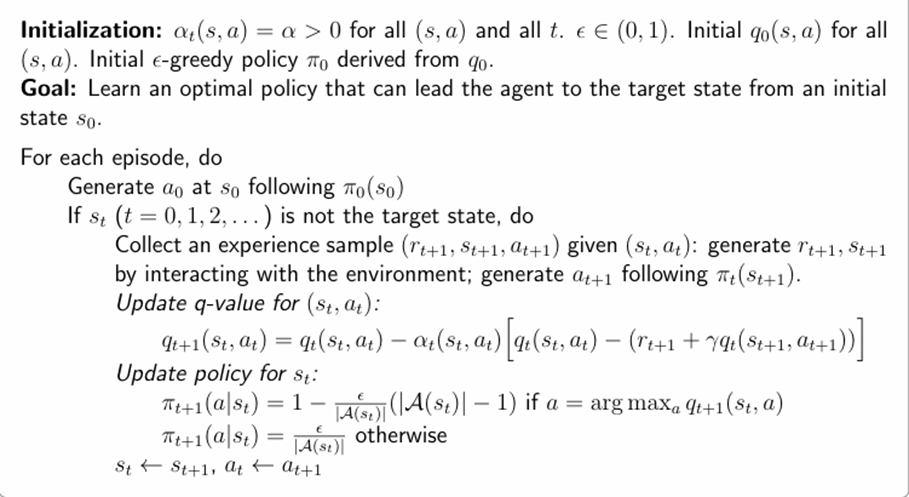
\includegraphics[]{images/sarsa.png}
  \caption{sarsa}\label{fig:sarsa}
\end{figure}

\textcolor{black}{目标:学习最优策略,使智能体能从给定状态$s_{0}$到达目标状态。}

\textcolor{black}{对于图2-1中的Sarsa算法描述如下所示:}

\textcolor{black}{算法初始化:}

\textcolor{black}{对于所有$\left({s,a}\right)$数值和所有$t$数值,选取学习率因子${\alpha}_{t}\left({s,a}\right) = {\alpha}$,贪婪因子${\epsilon}\in({0,1})$,并且设定所有$\left({s,a}\right)$的初始值为${q}_{0}\left({s,a}\right)$,从${q}_{0}$获取初始贪婪策略${\pi}_{0}$。}

\textcolor{black}{算法目标:学习最优策略,使智能体能从给定的状态${s}_{0}$出发,到达目标终止状态。}

\textcolor{black}{对于每个回合:}

\textcolor{black}{\ \ 如果当前状态是${s}_{0}$根据$ {\pi}_{0}\left({s}_{0}\right)$,选取策略 $a ={a}_{0}$}

\textcolor{black}{\ \  在时刻t,如果${s}_{t}$不是目标状态}

\textcolor{black}{\ \ \ \  收集经验样本$({s}_{t}, {a}_{t}, {s}_{{t+1}}, {a}_{{t+1}})$:在${s}_{t}$通过与环境交互生成${r}_{{t+1}},{s}_{{t+1}}$。}

\textcolor{black}{\ \ \ \ 再根据${\pi}_{t}\left({s}_{{t+1}}\right)$生成 ${a}_{{t+1}}$}

\textcolor{black}{\ \ \ \  随后更新$({s}_{t}, {a}_{t})$的值}

\textcolor{black}{Sarsa算法也存在一些推广,例如Expected Sarsa算法、n-step Sarsa算法等,尽管本实验中并未涉及到这些推广算法,但是读者在构建强化学习对抗性样本生成模型上也可以尝试使用它们。}

\textcolor{black}{其中Expected Sarsa算法类似Sarsa算法,但是它们的时序差分方法目标上不同。具体实现流程上二者相似。}

\textcolor{black}{已知策略$\pi$,则Expected Sarsa算法对于该策略$\pi$的动作值估计公式如式(2-6)所示:}
\begin{equation}
q_{t+1}(s_{t},a_{t})=q_{t}(s_{t},a_{t})-\alpha _{t}(s_{t},a_{t})[q_{t}(s_{t},a_{t})-(r_{t+1}+\gamma E[q_{t}(s_{t+1},a_{t+1})]) 
\end{equation}

\textcolor{black}{\ $q_{t+1}(s,a)=q_{t}(s,a) \ while \ (s,a) \neq (s_{t},a_{t})$}
%%
% BIThesis 本科毕业设计论文模板 —— 使用 XeLaTeX 编译 The BIThesis Template for Undergraduate Thesis
% This file has no copyright assigned and is placed in the Public Domain.
%%

% 第一章节
\chapter{一级题目}

\section{二级题目}
% 这里插入一个参考文献,仅作参考

\subsection{三级题目}

正文……\parencite{ref1}……\cite{ref2}

\textcolor{blue}{正文部分:宋体、小四;正文行距:22磅;间距段前段后均为0行。阅后删除此段。}

\textcolor{blue}{图、表居中,图注标在图下方,表头标在表上方,宋体、五号、居中,1.25倍行距,间距段前段后均为0行,图表与上下文之间各空一行。阅后删除此段。}

\textcolor{blue}{\underline{\underline{图-示例:(阅后删除此段)}}}


\begin{figure}[htbp]
  \centering
  
\includegraphics[]{images/bit_logo.png}
  \caption{标题序号}\label{标题序号} % label 用来在文中索引
\end{figure}

\textcolor{blue}{\underline{\underline{表-示例:(阅后删除此段)}}}
% 三线表
\begin{table}[htbp]
  \centering
  \caption{统计表}\label{统计表}
  \begin{tabular}{*{5}{>{\centering\arraybackslash}p{2cm}}} \toprule
    项目    & 产量    & 销量    & 产值   & 比重    \\ \midrule
    手机    & 1000  & 10000 & 500  & 50\%  \\
    计算机   & 5500  & 5000  & 220  & 22\%  \\
    笔记本电脑 & 1100  & 1000  & 280  & 28\%  \\ \midrule
    合计    & 17600 & 16000 & 1000 & 100\% \\ \bottomrule
    \end{tabular}
\end{table}

\textcolor{blue}{公式标注应于该公式所在行的最右侧。对于较长的公式只可在符号处(+、-、*、/、$\leqslant$ $\geqslant$ 等)转行。在文中引用公式时,在标号前加“式”,如式(1-2)。阅后删除此
段。}

\textcolor{blue}{公式-示例:(阅后删除此段)}
% 公式上下不要空行,置于同一个段落下即可,否则上下距离会出现高度不一致的问题
\begin{equation}
    LRI=1\ ∕\ \sqrt{1+{\left(\frac{{\mu }_{R}}{{\mu }_{s}}\right)}^{2}{\left(\frac{{\delta }_{R}}{{\delta }_{s}}\right)}^{2}}
\end{equation}


\section{字体效果表格}

% 列:Regular、Italic、Bold、Bold Italic
% 行:宋体、黑体、楷体、Serif、Sans Serif、Typewriter、Math

\begin{table}[htb]
    \centering
    \caption{字体效果表格}
    \begin{tabular}{@{}lllll@{}}
    \toprule
               & Regular & Bold & Italic & Bold Italic \\ \midrule
      宋体       & 宋体      & \colorbox{orange}{\textbf{宋体粗体}} & \textit{楷体}     &   \colorbox{gray}{\textbf{\textit{楷书粗斜体}}}  \\
      黑体         & {\heiti{}黑体}      & \textbf{\heiti{}黑体粗体} &   \textit{\heiti{}黑体斜体}     & \colorbox{gray}{\textit{\textbf{\heiti{}黑体粗斜体}}}   \\
      楷体         & {\kaishu{}楷书}      & \textbf{\kaishu{}楷书粗体} & \textit{\kaishu{}斜体楷体} &  \colorbox{gray}{\textbf{\textit{\kaishu{}楷书粗斜体}}}    \\
    Serif(Roman/Normal)      &    Regular    &  \textbf{Bold}  &    \textit{Italic}    &     \textbf{\textit{Bold Italic}}    \\
    Sans Serif &  \textsf{Regular}       &  \textbf{\textsf{Bold}}    &  \textit{\textsf{Bold}}   &    \textbf{\textit{\textsf{Bold}}}   \\
    % 有些字体缺少特定变体,LaTeX会抛出警告,同时尽量替换为相近变体。
    % 若编译结果能接受,可忽略之。
    % 例如此处Typewriter代表的Latin Modern Sans Typewriter(lmtt)字体没有bold extended italic(bx/it)变体,
    % 所以`\textbf{\textit{\texttt{…}}}`会被替换为bold slant(b/sl)变体,并引发如下警告。(其中TU指字体编码)
    % Font shape `TU/lmtt/bx/it' in size <…> not available. Font shape `TU/lmtt/b/sl' tried instead.
    Typewriter &  \texttt{Regular}       &  \textbf{\texttt{Bold}}    &  \textit{\texttt{Bold}}   &    \textbf{\textit{\texttt{Bold}}}   \\
    Math       &   $\mathnormal{Regular} \mathrm{Roman}$  & $\mathbf{Bold}$   &    $\mathit{Italic}$    &  $\mathbf{\mathit{Bold Italic}}$    \\ \bottomrule
    \end{tabular}
\end{table}

\begin{itemize}[nosep]
  \item \colorbox{orange}{宋体粗体}在 Windows 下会成为黑体。这是因为 Windows 的中易宋体没有粗体字重而进行的妥协。
    如果想要获得宋体粗体的样式,请在配置中开启伪粗体选项。
  \item \colorbox{gray}{粗斜体}的效果是因操作系统字体而定的,中文写作中不会使用这种字形,可以忽略。
\end{itemize}

\textit{有关公式与上下文间距的一些注意事项:请保证源码中的公式的环境(如}
\\ \verb|\begin{equation}|
  \textit{)与上一段落不要有空行。否则,公式和上文段落之间会有额外的空白。}


\section{常见问题和疑难解答}

如果您遇到\href{https://bithesis.bitnp.net/faq/char-missing.html}{生僻字无法显示}、
\href{https://bithesis.bitnp.net/faq/enumitem-nosep.html}{列表项间距过大}、
\href{https://bithesis.bitnp.net/faq/longtable.html}{三线表需要跨页}等问题,
请参考\textcolor{magenta}{\href{https://bithesis.bitnp.net/faq/}{在线文档的「疑难杂症」部分}}。

%%
% BIThesis 本科毕业设计论文模板 —— 使用 XeLaTeX 编译 The BIThesis Template for Undergraduate Thesis
% This file has no copyright assigned and is placed in the Public Domain.
%%

\chapter{另一个章节}

\section{代码片段}

\begin{lstlisting}[language=Python, caption={Python Code}, label={lst:pythonfile}]
import numpy as np

def incmatrix(genl1,genl2):
    m = len(genl1)
    n = len(genl2)
    M = None #to become the incidence matrix
    VT = np.zeros((n*m,1), int)  #dummy variable

    #compute the bitwise xor matrix
    M1 = bitxormatrix(genl1)
    M2 = np.triu(bitxormatrix(genl2),1)

    for i in range(m-1):
        for j in range(i+1, m):
            [r,c] = np.where(M2 == M1[i,j])
            for k in range(len(r)):
                VT[(i)*n + r[k]] = 1;
                VT[(i)*n + c[k]] = 1;
                VT[(j)*n + r[k]] = 1;
                VT[(j)*n + c[k]] = 1;

                if M is None:
                    M = np.copy(VT)
                else:
                    M = np.concatenate((M, VT), 1)

                VT = np.zeros((n*m,1), int)

    return M
\end{lstlisting}


% 后置内容
\backmatter

% 结论:在相应 TeX 文件撰写
%%
% BIThesis 本科毕业设计论文模板 —— 使用 XeLaTeX 编译 The BIThesis Template for Undergraduate Thesis
% This file has no copyright assigned and is placed in the Public Domain.
%%

\begin{conclusion}
  % 结论部分尽量不使用 \subsection 二级标题,只使用 \section 一级标题

  % 这里插入一个参考文献,仅作参考
\textcolor{black}{本实验使用了Sarsa算法构建了一个强化学习的静态查杀规避处理框架,用于生成对一些黑盒的反病毒软件和反病毒引擎的对抗性扰动静态规避攻击样本,动作选择可以认为是多臂老虎机问题,在有限的尝试次数下探索较好的行为,尽量规避无效动作,降低修改总次数来实现规避概率最大化。实验表明,处理前后在Clam AV和火绒杀毒下检出率变化较小,这可能是因为这两款杀毒软件自带一定的抗扰动能力,能对抗本实验中对于恶意软件的针对静态检测的扰动处理,然而360杀毒的云查杀引擎在没有云上传功能下,对处理后的恶意软件样本查杀率很低。实验表明了,在采用相似检测机制的反病毒软件之间,该模型具有可迁移攻击特性,且能推测出QVM反病毒引擎的抗扰动能力较弱,说明部分基于机器学习的反病毒引擎仍然有待升级。本实验的对抗性样本生成强化学习框架在基于原有的GYM-Malware,PSP-Malware,Mab-Malware基础上,尝试了新的强化学习算法,并且降低了模块之间的耦合性,便于后续的研究人员利用已有的研究成果创建新的强化学习框架。}
\textcolor{black}{同时本实验中也存在着一些不足:}

\textcolor{black}{(1)使用的机器性能问题,为避免程序崩溃,Sarsa算法允许的最大步数上限不能调的很高,导致可能存在一些样本,这些样本再经过一些操作也能达到规避静态检测,但智能体在指定步数之内会判定扰动产生的对抗性样本无效。}

\textcolor{black}{(2)最后,本实验尚未考虑到Windows下其它恶意程序的对抗性样本生成,例如恶意shellcode,恶意JavaScript代码等。}
\end{conclusion}

% 参考文献:
% 添加文献时,请按 BibTeX 格式添加至 misc/ref.bib,并在正文所需位置使用 \cite{…} 引用。
% 如无特殊需要,无需改动相应 TeX 文件。
%%
% BIThesis 本科毕业设计论文模板 —— 使用 XeLaTeX 编译 The BIThesis Template for Undergraduate Thesis
% This file has no copyright assigned and is placed in the Public Domain.
%%

% 如无特殊需要,本页面无需更改

\begin{bibprint}

\printbibliography[heading=none]

\end{bibprint}

% 附录:在相应 TeX 文件撰写;不需要时可删除
%%
% BIThesis 本科毕业设计论文模板 —— 使用 XeLaTeX 编译 The BIThesis Template for Undergraduate Thesis
% This file has no copyright assigned and is placed in the Public Domain.
%%

\begin{appendices}
\textcolor{black}{本实验中关于强化学习的内容,部分参考了赵世钰老师的《强化学习的数学原理》中文译本,其英文原本位于https://github.com/MathFoundationRL/Book-Mathematical-Foundation-of-Reinforcement-Learning,感兴趣的读者可以去学习其它的强化学习算法,例如值函数方法和策略梯度方法,以及演员-评论家方法,本文限于篇幅以及本实验中没有涉及到这些强化学习算法在此不予给出,读者可以参考该中文译本来进行对强化学习的进一步学习。}

\textcolor{black}{本实验的相关代码遵循MIT开源协议,笔者已经将代码上传到了GitHub上,项目地址是:https://github.com/Oldmemory1/GraduateDesign/tree/master }

\end{appendices}

% 致谢:在相应 TeX 文件撰写
%%
% BIThesis 本科毕业设计论文模板 —— 使用 XeLaTeX 编译 The BIThesis Template for Undergraduate Thesis
% This file has no copyright assigned and is placed in the Public Domain.
%%

% 致谢部分尽量不使用 \subsection 二级标题,只使用 \section 一级标题
\begin{acknowledgements}
  值此论文完成之际,首先向我的导师……

  \textcolor{blue}{致谢正文样式与文章正文相同:宋体、小四;行距:22 磅;间距段前段后均为 0 行。阅后删除此段。}
\end{acknowledgements}


\end{document}
